\section{TSTL Tools}
\label{sec:tools}

The following tools are provided in the TSTL distribution on github \cite{tstl}.  Installing the TSTL module allows the compiler, called {\tt tstl}, to be used at the command line.  Other tools are included in the {\tt generators} and {\tt utilities} directories of the distribution as Python scripts.

\subsection{The TSTL Compiler}

Given a harness file defined in the language discussed above, the TSTL compiler generates a stand-alone Python class that allows testing of the SUT.  This generated code does not depend on the TSTL system being installed, only on any modules the testing itself uses, and on whether code coverage is requested.  By default, the compiler produces a class supporting code coverage using the {\tt coverage.py} module \cite{coveragepy}, and assumes this is installed.  The TSTL compiler also allows a user to control some fine-grained coverage measures (e.g, is coverage measured during initialization and module reloads?), and force a system to use replay-based backtracking by default.

\subsection{Test Generators}

TSTL comes with a complex, highly configurable, pure random tester (supporting numerous command-line options).  The included random tester provides a number of useful options, of which a subset are shown in Figure \ref{tab:rt}.   

\begin{figure}
{\scriptsize
\begin{itemize}
\item {\tt depth <int>}: Determines the length of generated tests.
\item {\tt timeout <int>}: Determines the maximum time spent generating tests, in seconds.
\item {\tt seed <int>}: Determines the random seed for testing.
\item {\tt maxTests <int>}: Determines the maximum number of tests to be generated.
\item {\tt running}: Produce on-the-fly, time-stamped code coverage information, for analyzing performance of testing algorithms. 
\item {\tt replayable}: Produce a log of the current test, so even it crashes Python the test can be reproduced, delta-debugged, made stand-alone, or otherwise analyzed.
\item {\tt total}: Produce a total log of all test activity, including across resets, for systems where reset is not complete (so tests across resets can be delta-debugged).
\item {\tt quickTests}:  Produce ``quick test'' files \cite{icst14}, each containing a minimal test to cover a set of branches of the SUT. 
\item {\tt normalize}: Apply additional, custom term-rewriting based simplifications of test cases that often further minimize delta-debugged test cases. 
\item {\tt generalize}: Apply generalization that elaborates each failing test with annotations showing similar tests that also fail. 
\item {\tt swarm:}  Apply swarm testing \cite{ISSTA12} to test generation.
\end{itemize}
}
\caption{Some options for the TSTL random test generator.}
\label{tab:rt}
\end{figure}

To our knowledge, TSTL's random tester is the first general-purpose random testing tool to incorporate the powerful swarm testing \cite{ISSTA12} algorithm, which has previously been used to test compilers \cite{ISSTA13,ZhendongPLDI14} and file systems.  TSTL's version of swarm testing is more sophisticated than previously published versions, in that it analyzes the dependency graph of TSTL actions to avoid producing degenerate test configurations, improving performance over na\"ive swarm testing.  In addition to these stable, commonly used options, the random tester includes novel experimental options, such as the ability to guide random testing by a user supplied Markov model or operational profile \cite{Hamlet94}.  TSTL makes implementing novel test generation methods simple, as discussed below.

The base TSTL tools also use the TSTL interface to support explicit-state model-checking \cite{ModelChecking,SPIN}, using either Depth-First-Search (DFS) or Breadth-First-Search (BFS) strategies.  TSTL uses Python's {\tt deepcopy} tools to provide a simple, easy to use interface for automatically storing and restoring pool states, making these algorithms trivial to implement.  There is no fundamental technical difference between performing (theoretically exhaustive) systematic searches of a well-defined transition system or random exploration.  Using the same transition system definition for both purposes has considerable advantages, as pointed out in previous work \cite{woda08}, especially for effectively infinite-state systems where random walks will never saturate and exhaustive searches will never complete.
TSTL can (unlike SPIN or most explicit-state model checkers) apply BFS or DFS search even to systems without support for backtracking.  TSTL's abstract interface to an SUT (transition system) can be configured to provide replay-based simulation of state storage and retrieval.  This is required when, for example, a library uses a C extension and so Python's {\tt deepcopy} does not allow full copying of the state of pool objects, or when the system has hidden global state that cannot be captured in a pool value.  While state storage and backtracking is usually faster than replay, we find that for some systems the opposite is true, particularly for shallow search depths (which are typical for BFS of a complex system).

TSTL also supports custom abstraction of pools.  If a pool is declared with an {\tt ABSTRACT} annotation, the function after the {\tt ABSTRACT} keyword is used to abstract all values for state-matching purposes during exhaustive exploration methods, via the {\tt abstract} function.  The {\tt state} method returns the concrete state of the system (since these are required for backtracking), but applying the {\tt abstract} function to this state returns an abstract version of the state to be used in state matching.  The core of a BFS, for example, can be expressed quite simply, irrespective of whether the system is using state storage and backtracking or replay (or has an abstraction or not) as:

{\scriptsize 
\begin{code}
old = sut.state()
for act in sut.enabled():
   sut.safely(act)
   new = sut.state()
   \# repr produces a hashable string representation
   absNew = repr(sut.abstract(new))
   if absNew not in visited:
      queue.append(new)
      visited[absNew] = True
      ...
   sut.backtrack(old)
\end{code}
}

This loop iterates through all enabled actions from the current state, and adds any not previously visited to the search queue.  Similar code works as the core of a DFS.  Implementing heuristic model checking searches is also trivial, whether those searches are SUT/error specific \cite{EdelkampHeur} or structural \cite{groce-structural}.

While not required for any of our testing efforts thus far, encoding temporal logic checking is also simple.  A B\"uchi automata can be encoded in Python, querying the SUT state and action choices to determine transitions.  Composing this with the SUT state is trivial.  We managed to implement the well-known nested DFS algorithm \cite{DoubleDFS} in less than 40 lines of code, taking the property automata as a tuple input {\tt(initial, trans, accept)}, where {\tt trans: (state, action, sut state) -> state}.

\subsection{Utilities for Test Case Manipulation}

TSTL provides the tools {\tt sandboxreducer} and {\tt standalone} for manipulating saved test cases produced by the random tester or the simple model checkers.  These were developed as part of the ArcPy testing process.  ArcPy faults tend to crash the system (this is also the reason the {\tt total} option was introduced), and thus cannot be simplified for debugging inside the test generator.   The sandbox reducer takes a testing log and, using subprocesses to handle crashes, produces delta-debugged and normalized test cases. It is also useful to report failing tests not as TSTL's internal test file format, but as standalone Python programs that cause a failure.  The {\tt standalone} utility takes a test log or a saved test case and produces a complete, stand-alone Python program that requires neither the generated TSTL interface nor any other TSTL tools.

\begin{figure}
{\scriptsize
\begin{code}
import sut
import glob

sut = sut.sut()

failed = 0
total = 0

for testFile in glob('regressions\\*.test'):
   t = sut.loadTest(testFile)
   total += 1
   if sut.failsAny(t):
       failed += 1
       print testFile,'FAILED:',sut.failure()

print total,'TESTS EXECUTED'
print failed,'TESTS FAILED'

print len(sut.allBranches()),'BRANCHES COVERED'
print len(sut.allStatements()),'STATEMENTS COVERED'
print sut.report('coverage.txt'),'\% STATEMENTS COVERED'
\end{code}
}
\caption{A small script to run stored regression tests}
\label{fig:regress}
\end{figure}


However, use of these tools is often not required.  Figure \ref{fig:regress} shows a simple, but complete, Python script for running regression tests generated using TSTL for a system.  This script examines the {\tt regressions} directory, replays each test in the directory, and reports on failing tests and code coverage.  Such a script can easily be customized to provide different tests for different budgets (e.g., prioritized by time, coverage, or to execute coverage-based 'quick tests').

\subsubsection{ArcPy Regression Generation}

One difficulty for ArcPy users is ensuring that their existing scripts
and tools work on new versions of ArcGIS.  Each recent major release
(10.2 and 10.3) after ArcPy's introduction has potentially included some changes
in the behavior of API calls.  Detecting when such changes cause a
script to break is difficult.  A first step would be an automatic way
to find when the return values for calls differ between ArcPy
versions.
Because installing multiple versions of ArcGIS on the same system is
difficult or impossible, our method for finding differences relies on
choosing a reference version (10.3 in our current efforts), and
generating a set of standalone tests that 1) cover a large amount of
ArcPy functionality, including invalid inputs to functions and 2)
record the return values and exceptions raised by calls.  These tests
can be run on any ArcPy version, and will report differences between
the tests and version 10.3.  Performing this kind of differential
testing \cite{Differential} on old or new major releases, or across 64
bit and 32 bit versions, is easy.  In the long run, we also want to
enable TSTL to produce Python 3.0+ code, for use with ArcGIS Pro,
which uses Python 3.4 instead of 2.7.  This has motivated a branch to
TSTL to support Python 3.0 (unfortunately, Python 3.0 is not fully
backwards compatible with earlier versions, Python 2.7 is still
the most widely used Python, and non-pro versions of ArcPy \emph{only} work
with 2.7).

We generate coverage-based regression tests using an approach called \emph{quick
  testing} \cite{icst14,stvrcausereduce}, which takes a set of tests
produced by random testing or model checking, and applies a test case reduction
algorithm \cite{DD} to produce smaller tests that have the same code
coverage as the very large, highly redundant, original set of test
cases.  Automatic quick-testing was added to TSTL's random test
generator to support ArcPy testing.  Combined with standalone test
generation, this allows us to produce test cases that can be run on
any version of ArcPy, and explore a large variety of behavior of the
code.  With ArcPy, coverage alone, unlike previous quick testing
efforts, is insufficient to ensure a useful regression test.  Because
coverage only considers the Python behavior of ArcPy (since we do not
have access to the source for the ArcGIS engine), it may group
behaviors that are not similar together.  We added the ability to
combine coverage preservation with preservation of all ArcPy messages
indicating a successful GIS engine operation, after abstracting away
such details as the runtime of the operation, and so forth.

However, just producing these coverage-and-engine-behavior preserving
standalone tests is not sufficient for good version comparison, since
standalone test cases as produced only check for properties defined in TSTL.  An
additional option was added to the standalone test generator, allowing
it to record the actual return values of all calls, the set of
exceptions thrown, the success/failure messages from the ArcPy engine, and so forth to more precisely record a test's
behavior on an ArcPy version.


\subsection{Visualization of Action Spaces}

\begin{figure}
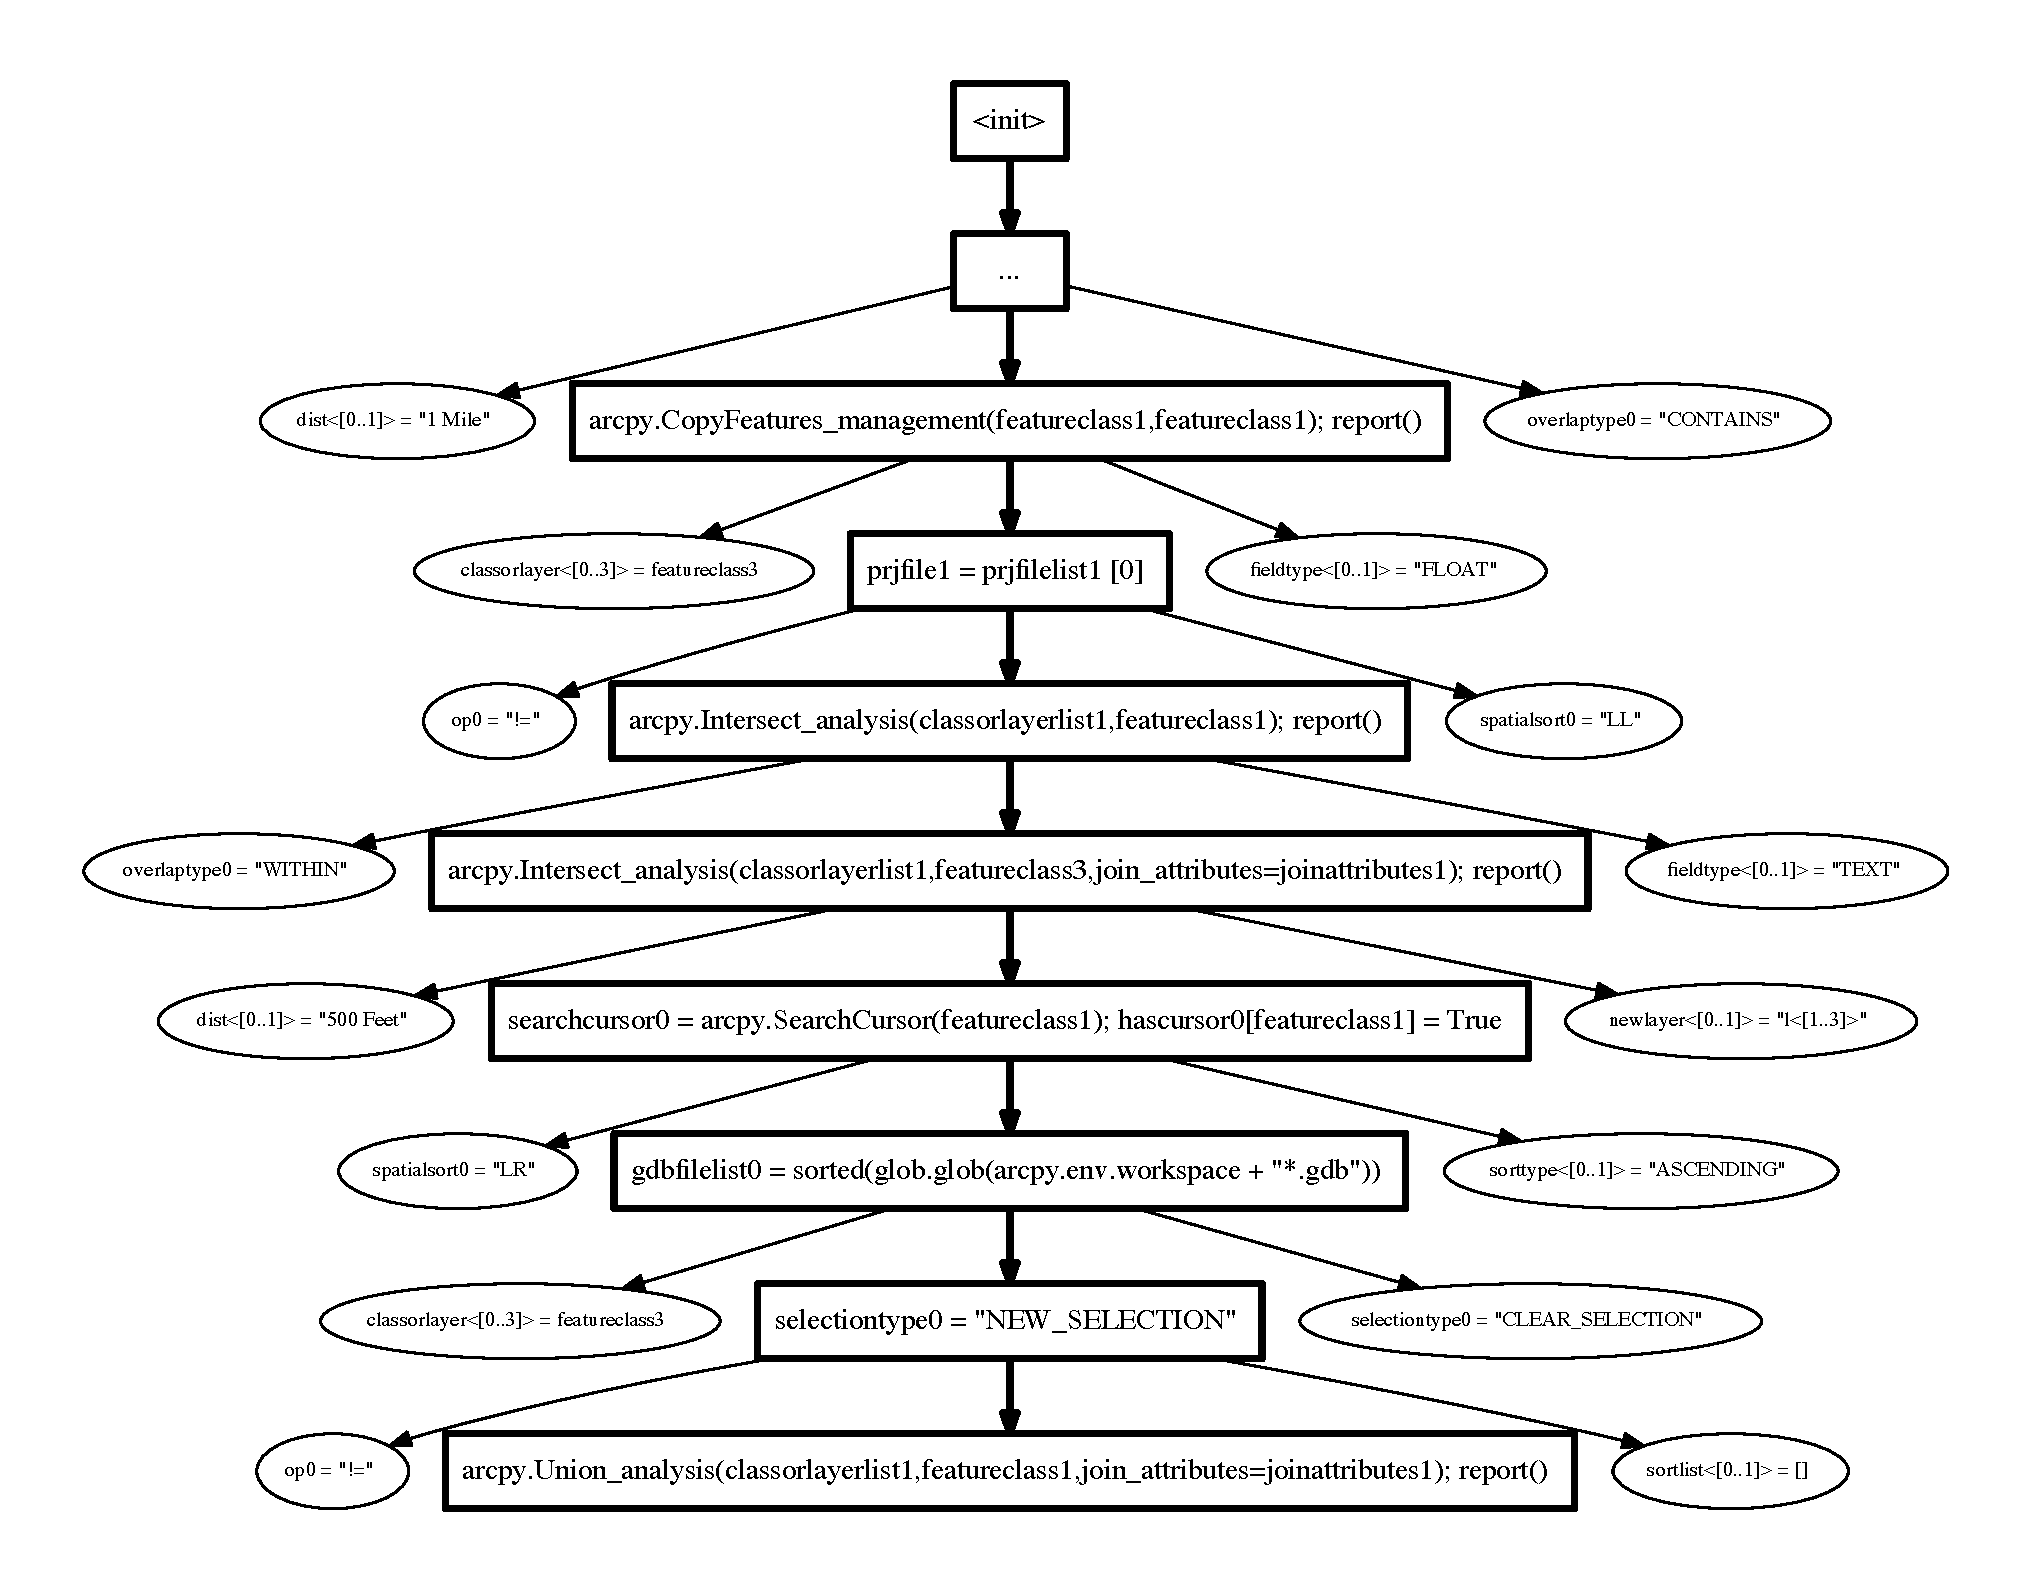
\includegraphics[width=\columnwidth]{shortgraph}
\caption{Start depth 20, depth 8, width 3 trace visualization for ArcPy testing.}
\label{fig:actions}
\end{figure}

Understanding the structure of the action graph produced by even a relatively simple TSTL harness can be difficult.  The structure is often infinite, and even in cases where there is a finite state space (perhaps introduced by abstraction) the graph is usually far too large for a convenient display.  However, we have found that a visual representation of typical trajectories through the system can be very helpful for understanding a complex test system.  The {\tt makegraph} utility takes as input a number of traces to produce, a starting depth, additional depth, and a test width.  It then produces in pdf form a number of graphs for traces like the one shown in Figure \ref{fig:actions}.  These trace graphs show, in bold, the actual action sequence chosen by a pure random tester, starting after a number of actions not shown (represented by the ``...'' node) and continuing up to the depth limit.  In addition to the actions taken, the graph also shows a random subset of additional enabled actions, with each step showing a number of actions equal to the width.  Because many actions are extremely similar, the graphing utility also summarizes actions that are the same, except for pool choice or integer constant, using the {\tt <[i..j]>} notation of TSTL.

\subsection{Building Your Own Testing Tools in TSTL}
\label{sec:build}

Describing the full interface provided by TSTL for use in testing tools is beyond the scope of this paper.  However, examining the source code of the included testers can provide a good starting point.  Implementing new test case manipulations usually involves understanding TSTL internal structures and how tests are stored.  Implementing novel test generation algorithms can often rely on just a handful of methods, shown in Figure \ref{methods} (TSTL provides nearly 100 methods for generating and manipulating tests, but this minimal set can implement many test generation algorithms).

\begin{figure}
{\scriptsize
\begin{itemize}
\item {\bf restart():}  resets the system state and aborts the current test. 
\item {\bf test():} returns the current test.
\item {\bf replay(test):} replays a test, and returns a Boolean indicating success or failure of the test.
\item {\bf enabled():} returns a list of all currently enabled actions.
\item {\bf randomEnabled(random):}  given a Python random number generator object, returns a random enabled action, efficiently (avoiding unnecessary guard evaluations).
\item {\bf safely(action):} performs action (usually changing SUT state)  and returns a Boolean indicating whether the action performed raised any uncaught exceptions. 
\item {\bf check():} returns a Boolean indicating whether any properties fail for the current state.
\item {\bf error():} returns either {\tt None} (no error for the last action or {\tt check}), or a Python object representing an uncaught exception or failed property's backtrace.
\item {\bf state():} returns the current SUT state, as a set of values for all pools; for systems where state cannot be restored by pool values, or {\tt deepcopy} does not work, returns the current test.
\item {\bf backtrack(state):} takes a state or test produced by {\tt state} and restores the system to it.
\item {\bf reduce(test,predicate):} takes a test and a predicate (function from test to boolean), and returns a (possibly smaller) test also satisfying the predicate.
\item {\bf allBranches():} returns the set of branches covered during all testing.
\item {\bf newBranches():} returns the set of branches covered during the last action executed that had not previously been covered.
\item {\bf currBranches():} returns the set of branches covered during the current test.
\item {\bf saveTest(test, filename):} saves a test in a file.
\item {\bf loadTest(filename):} loads a test from a file (and returns that test as the function's return value).
\end{itemize} 
}
\caption{Some core methods for testing an SUT.}
\label{methods}
\end{figure}

For example, a researcher aware of the literature showing that for many systems it is difficult to outperform random testing, due to its very low overhead \cite{ISSRE12,ISSTA12}, may consider simple modifications of random testing that do not greatly increase overhead.  One such example, with implementation, is shown in the original TSTL paper \cite{NFM15}.  We present another here.  Since the focus of this paper is on showing how to use TSTL, not novel test generation methods, we leave a complete development and statistically valid evaluation of our proposed approach to future work, but discuss briefly how to go about prototyping and evaluation using TSTL.

The idea is to perform random testing, but keep the final state of tests with unusually high coverage as potential starting points for future tests, potentially extending them far beyond the normal test length limit.  The approach is parameterized by {\tt MEMORY}, the number of ``good'' tests to store, by {\tt PEXTEND}, the probability of choosing to extend a ``good'' test rather than start a new test, by the {\tt TEST\_LENGTH} and by a {\tt TIMEOUT} parameter.  Leaving out imports and other boilerplate, the entire implementation is shown in Figure \ref{fig:keepgood}.

\begin{figure}
{\scriptsize
\begin{code}
goodTests = []
startTime = time.time()
while (time.time() - startTime <= TIMEOUT):
   if (len(goodTests) > 0) and (rgen.random() < PEXTEND):
     sut.backtrack(rgen.choice(goodTests)[1])
   else:
     sut.restart()
   for s in xrange(0,TEST\_LENGTH): 
      action = sut.randomEnabled(rgen)
      r = sut.safely(action)
      if len(sut.newBranches()) > 0:
         print time.time(),len(sut.allBranches()),'NEW BRANCHES:', sut.newBranches()
   if MEMORY > 0:
      goodTests.append((sut.currBranches(), sut.state()))
      goodTests = sorted(goodTests, reverse=True)[:MEMORY]
\end{code}
}
\caption{Implementing a very simple novel testing algorithm.}
\label{fig:keepgood}
\end{figure}

\begin{figure}
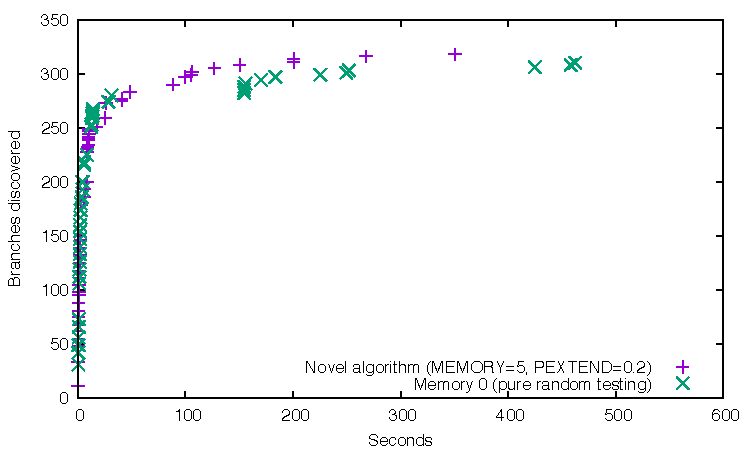
\includegraphics[width=\columnwidth]{memory}
\caption{Comparing branch coverage for 10 minute runs of two test generation methods.}
\label{fig:compare}
\end{figure}

The implementation is trivial, relying only on the TSTL API and some very simple Python tools (sorting with automatic lexical ordering, time library, etc.).  We omit handling of failed tests, assuming the goal of this algorithm is simply to improve code coverage in fault-free systems for experimental evaluation.  This simple tool can be applied to any TSTL harness and will produce output showing when, in time, new branches were covered by the system.  This data can be used to produce Average-Percent-Branches-Detected (APBD) values and discovery curves \cite{issta14,Rothermel1999,rothermel01oct}. Comparison with simple random testing is easy, since setting {\tt MEMORY} to 0 gives pure memoryless random testing (alternatively, to avoid the overhead of the comparisons with 0, a dedicated version for random testing can be written).  A major threat to validity in many comparisons of testing or explicit-state model checking algorithms is that different underlying infrastructure for different algorithms may end up outweighing even moderately sized effects due to the underlying algorithms.  With TSTL, fair comparisons are much easier, since the TSTL interface does most of the computational work that is common to multiple algorithms, with the same overhead.  Evaluating an algorithm can be as simple as finding a large number of suitable programs without failures (or where failures don't make coverage values invalid) and performing enough trials to establish statistical validity for comparisons with APBD values for known algorithms.  Evaluation in terms of discovered faults or time-until-discovery of a fault is nearly as simple.  This algorithm is of some interest, in that while it requires backtracking, the frequency of backtracking is low enough to be potentially applicable even to systems like ArcPy where backtracking is only possible via expensive test replay.  While a mature version of this method would require many SUTs and experiments, as well as investigation of suitable values for {\tt MEMORY} and {\tt PEXTEND}, Figure \ref{fig:compare} shows that average branch discovery curves for ArcPy can sometimes be improved, even using the  arbitrarily chosen parameters of a size 5 memory and a 20\% probability of using a ``good'' test as a starting point.  The simplicity of the Python implementation makes performing automatic experiments with different parameters and test lengths trivial.  Experiments can also take advantage of Python libraries for automatic statistical analysis and plotting of results.


\section{TSTL as a Testing Library Generator}
\label{sec:langext}

While TSTL is easily used as ``just another tool'' that allows testing of an SUT, plus a ``construction kit'' to build your own testing tools, TSTL can also be understood as a generator of libraries.  ArcPy is a site package that makes it easy to perform GIS tasks using Python.  NumPy \cite{NumPy} and SciPy \cite{SciPy} are libraries that make performing scientific computing tasks easy with Python.  QIIME \cite{QIIME}, Biopython \cite{biopython}, and scikit-bio \cite{scikitbio} are libraries that make performing bioinformatics tasks easy using Python.  Such libraries can be of great importance in their subject domains:  ArcPy is extremely widely used, and the subject of university courses in many GIS programs; the Nature Methods paper introducing QIIME has been cited more than 5,000 times to date, according to Google Scholar.  TSTL, also, can be seen as a tool that generates a library making it easy to perform testing tasks \emph{for a specific SUT}, using Python. 

ArcPy, NumPy, QIIME and the other libraries can be seen as introducing the entities essential to their respective tasks as first-class, easily manipulable objects in the Python language.  TSTL makes tests (for a specific SUT, but using a common interface across all SUTs) first-class, easily manipulable objects.  TSTL does for tests, SUT state, and code coverage what ArcPy does for feature classes, spatial references, and other GIS concepts, what NumPy does for efficiently represented arrays and matrices, and what QIIME does for protein sequences.

The key to understanding TSTL as a library generator is the idea of a test.  A TSTL test is a list of actions\footnote{We expect this type to be the same for any TSTL version for any language:  a list is the simplest way to express pure sequence, which is the essence of a test.}.  The individuals of the action type are dependent on the SUT.  TSTL allows the user to generate, manipulate, and inspect tests in the same way NumPy lets a user explore the behavior of arrays.  This means that TSTL can also be used interactively, as the following example (using some TSTL-supplied methods not shown in Table \ref{methods}) shows:

{\scriptsize
\begin{code}
 >>> import sut, random
 >>> sut = sut.sut()
 >>> r = random.Random()
 >>> (t1, ok) = sut.makeTest(100,r)
 >>> print ok
 True
 >>> sut.prettyPrintTest(t1)
 fieldname1 = "newf1"                                                      \# STEP 0
 polytable0 = arcpy.env.workspace + "\\polyneig.dbf"                        \# STEP 1
...
 arcpy.Erase\_analysis(classorlayer0,classorlayer1,featureclass0); report() \# STEP 98
 arcpy.Buffer\_analysis(classorlayer3,featureclass0,dist1); report()        \# STEP 99
\end{code}
}

Here, a user generates a length 100 test for ArcPy, and then prints it.  The user can also modify the test slightly, using standard Python list modification, generate another test, produce a third test that is the \emph{composition} of the first two tests, and reduce that third test to remove any redundant (with respect to code coverage) steps in it.

{\scriptsize
\begin{code}
 >>> t1[1] = sut.playable(t1[1][0].replace("newf1","newf2"))
 >>> (t2,ok) = sut.makeTest(100,r)
 >>> print ok
 True
 >>> t3 = t1 + t2
 >>> sut.replay(t3)
 >>> bc = sut.currBranches()
 >>> t4 = sut.reduce(t3, sut.coversBranches(bc))
 >>> len(t4)
 78
...
\end{code}
}

The user is causing ArcGIS to perform GIS operations, but without specifying those operations; the GIS tasks are conceptually reduced to the actions of an arbitrary SUT, but the printed test makes it clear what is going on at the SUT level.  While this example shows the {\tt makeTest} interface being used with the default generator (pure random testing), a user can supply a more complex generator as a function.  For example, to implement testing such that if the last action resulted in any new coverage, it is repeated, a user could first
define a generator function (assume that {\tt r} is a random number generator defined globally, as above):

{\scriptsize
\begin{code}
def repeatGen(state,sut):
   (lastAction, r) = state
   if (lastAction != None) and (len(sut.newBranches()) > 0) and (lastAction[1]()):
      return (lastAction, lastAction)
   newAction = sut.randomEnabled(r)
   return ((newAction, r), newAction)
\end{code}
}
and then generate a length 100 test using this strategy easily:
{\scriptsize
\begin{code}
 >>> (t5, ok) = sut.makeTest(100, sgenerator=repeatGen, initial=(None,r))
\end{code}
}

The function {\tt repeatGen} takes a state consisting of a single action (or {\tt None} initially) and a random number generator.  It then, if there is a {\tt lastAction}, and the last step of testing increased branch coverage, and the action is still enabled, returns that action as both the next action to perform and the new state of the generator.  Otherwise, it generates a random action, and returns that as the state and the action.

We do not believe such an interactive approach to testing is natural with most other tools that generate either model checking traces or method-call sequence tests.  In fact, the very idea of test case composition as shown in the first interactive code fragment may seem quite strange to users of either model checking or conventional unit tests.  Although TSTL tests are sequences of actions --- essentially small, deterministic programs with no inputs --- they can be interacted with and generated like tests in QuickCheck \cite{ClaessenH00} or Hypothesis \cite{hypothesis}, where tests are usually just function inputs (lists, data structures, etc.). This ease-of-use for exploratory testing is a primary reason TSTL was first implemented for Python, rather than a compiled language such as Java or C (hence the ``Scripting'' part of ``Template Scripting Testing Language'').  A Swift, Ruby, or Scala version would also provide a way to interact with tests in a simple, immediate, and basically ``functional'' way.

